\vspace{-2mm}
\section{Introduction}\label{sec:intro}
\vspace{-2mm}

Diffusion models have gained popularity as powerful generative models. Their applications extend beyond image generation to include natural language generation \citep{sahoo2024simple,shi2024simplified,lou2023discrete}, molecule generation \citep{jo2022score,vignac2022digress}, and biological (DNA, RNA, protein) sequence generation \citep{avdeyev2023dirichlet,stark2024dirichlet}. In each of these domains, diffusion models have been shown to be very effective at capturing complex natural distributions. However, in practice, we might not only want to generate \emph{realistic} samples, but to produce samples that optimize specific downstream reward functions while preserving naturalness by leveraging pre-trained models. For example, in computer vision, we might aim to generate natural images with high aesthetic and alignment scores \citep{black2023training,fan2023dpok}. In drug discovery, we may seek to generate valid molecules with high QED/SA/docking scores \citep{lee2023exploring,jin2018junction} or RNAs (such as mRNA vaccines \citep{cheng2023research}) with high translational efficiency and stability \citep{castillo2021machine,asrani2018optimization}, and regulatory DNAs that drives high cell-specificity of expression \citep{gosai2023machine,taskiran2024cell,lal2024reglm}.    

The optimization of downstream reward functions using pre-trained diffusion models has been approached in various ways. In our work, we focus on non-fine-tuning-based methods because fine-tuning generative models (e.g., when using classifier-free guidance \citep{ho2020denoising} or RL-based fine-tuning \citep{black2023training,fan2023dpok,uehara2024finetuning,clark2023directly,prabhudesai2023aligning}) often becomes computationally intensive, especially as pre-trained generative models grow larger in the era of ``foundation models''. Although classifier guidance and its variants (\textit{e.g.}, \citet{dhariwal2021diffusion,song2020score,chung2022diffusion,bansal2023universal,ho2022video}) have shown some success as non-fine-tuning methods in these settings, they face significant challenges. First, as they would require constructing \emph{differentiable} proxy models, they cannot directly incorporate useful \emph{non-differentiable} features (\textit{e.g.}, molecular/protein descriptors \citep{van2013benchmarking,ghiringhelli2015big,gainza2020deciphering}) or non-differentiable reward feedback (\textit{e.g.}, physics-based simulations such as Vina and Rosetta \citep{trott2010autodock,alhossary2015fast,alford2017rosetta}), which are particularly important in molecule design to optimize docking scores, stability, etc. This limitation also hinders the principled application of current classifier guidance methods to recently-developed discrete diffusion models \citep{austin2021structured,campbell2022continuous,lou2023discrete} (\textit{i.e.}, without transforming the discrete space into the Euclidean space). %


\begin{wrapfigure}{r}{0.48\textwidth}
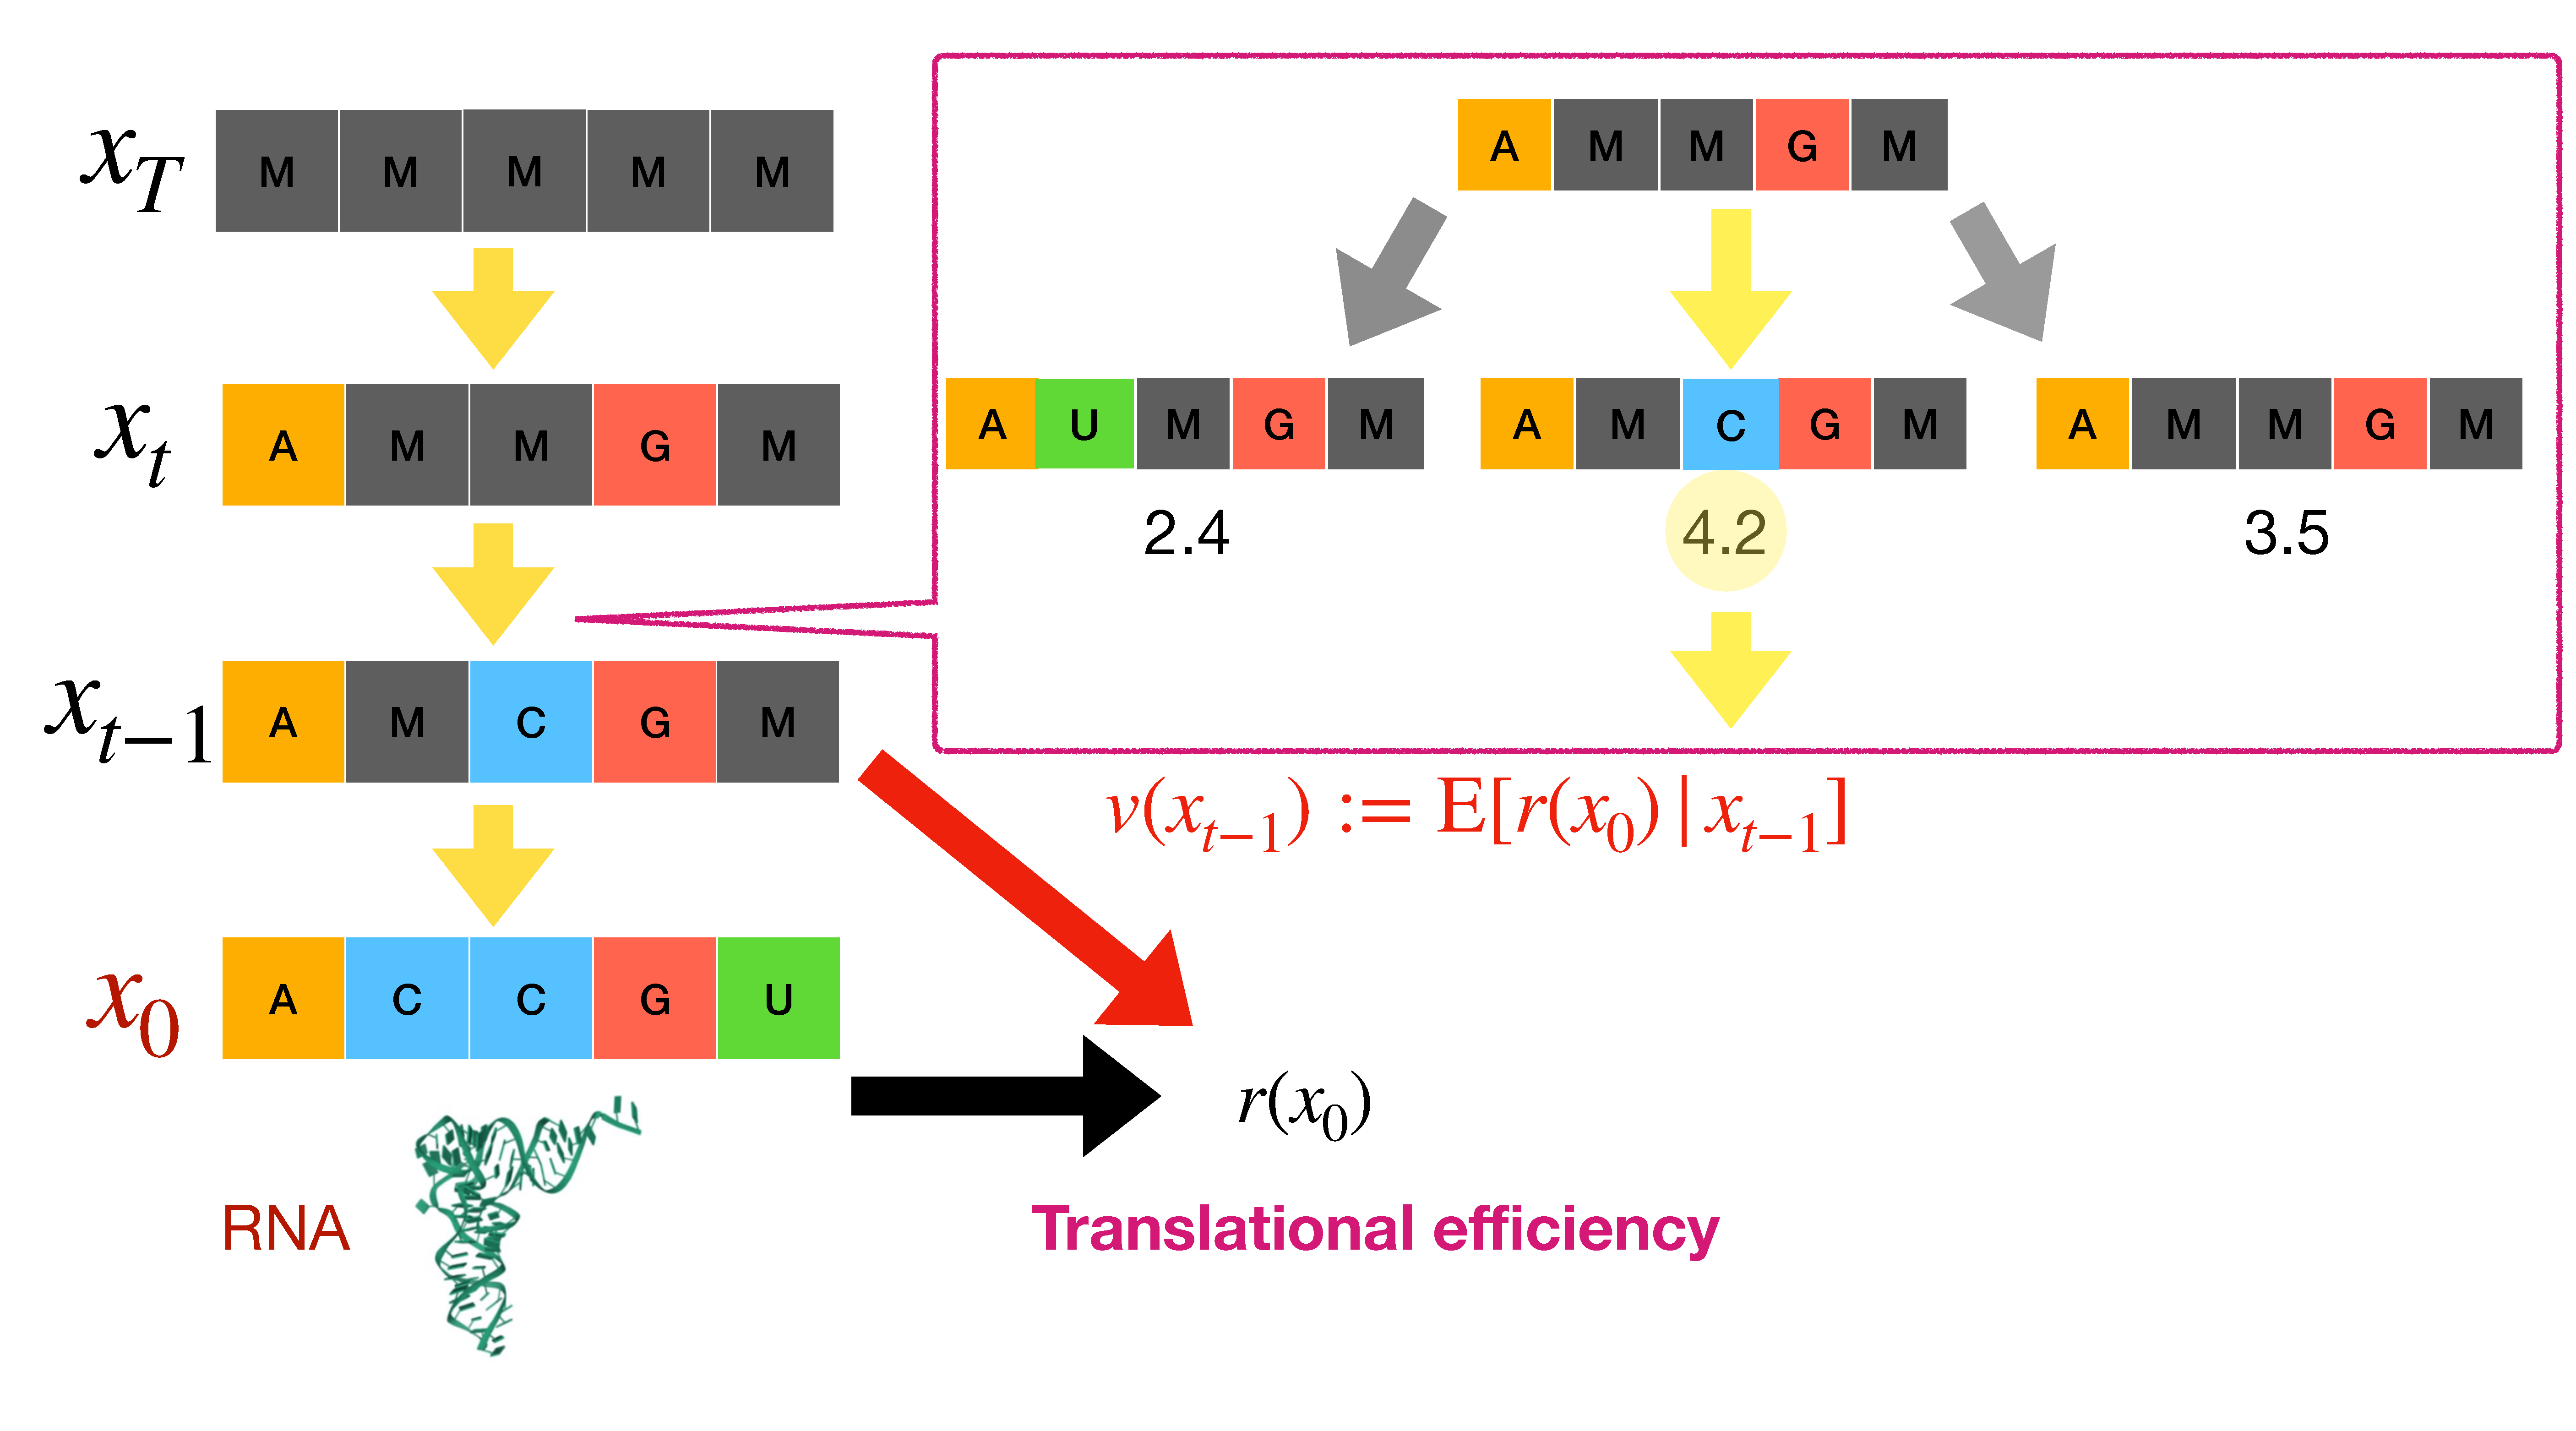
\includegraphics[width=0.48\textwidth]{images/Materials_up.pdf}
\caption{Summary of \alg. $v$ denotes value functions that predict reward $r(x_0)$ (at time $0$) from states at time $t-1$. {\alg} involves two steps: (1) generating multiple noisy states from pre-trained models, and (2) selecting the state with the highest value according to the value function.}
\label{fig:decoding}
\end{wrapfigure}



To tackle these challenges, we propose a novel method, \textbf{S}oft \text{V}alue-based \textbf{D}ecoding in \textbf{D}iffusion models (\alg), for optimizing downstream reward functions in diffusion models (\pref{fig:decoding}). Inspired by recent literature on RL-based fine-tuning \citep{uehara2024understanding}, we first introduce soft value functions that serve as look-ahead functions, indicating how intermediate noisy samples lead to high rewards in the \emph{future} of the diffusion denoising process.
After learning (or approximating) these value functions, we present a new inference-time technique, \alg, which obtains multiple noisy states from the policy (\textit{i.e.}, denoising map) of pre-trained diffusion models and selects the sample with the highest value function at each time step. Specifically, we introduce two algorithms (\alg-MC and \alg-PM) depending on how we estimate value functions. Notably, the \alg-PM approach does not require any additional learning as long as we have access to the reward feedback by utilizing the characteristics of diffusion models { (\textit{i.e.,} the forward process in diffusion models to directly map $t$ to $0$ in terms of expectation in \pref{fig:decoding}). }
  

\begin{table}[!t]
    \centering
        \caption{A comparison of \alg\,to prior approaches. ``Non-differentiable'' refers to the method's ability to operate without requiring differentiable proxy models. ``No Training'' means that no additional training of the diffusion model is required as long as we have access to the reward feedback. We compare to SMC-based methods in \pref{sec:TDS}. 
        } 
        \vspace{1mm}
        \scalebox{0.9}{ 
    \begin{tabular}{cccc}
         &       No fine-tuning    & Non-differentiable & No Training 
         \\ \midrule
     Classifier guidance    &  $\checkmark$ &    &       \\
     DPS \citep{chung2022diffusion}  & $\checkmark$  &    &   $\checkmark$    \\
     Classifier-free    &  & $\checkmark$    &    \\ 
     RL fine-tuning  &    & $\checkmark$  &     \\ 
    \rowcolor{Gray}   \alg-MC\,(here)   &$\checkmark$      & $\checkmark$   &    \\ 
     \rowcolor{Gray}   \alg-PM\,(here)   & $\checkmark$      & $\checkmark$   & $\checkmark$  
    \\ \bottomrule
    \end{tabular}
    } 
    \label{tab:summary}
    \vspace{-6mm}
\end{table}


 Our novel technique for optimizing downstream reward functions in pre-trained diffusion models makes two contributions (Table~\ref{tab:summary}). First, it eliminates the need {to construct differentiable proxy models}. This allows for the use of non-differentiable reward feedback, which is common in many scientific fields, and makes our method applicable to recent discrete diffusion \citep{shi2024simplified,sahoo2024simple} models without any modification. Second, it avoids the need to fine-tune the generative model itself.
 This addresses the high computational cost associated with fine-tuning diffusion models. We demonstrate the effectiveness of our methods across diverse domains, including image generation, molecule generation (optimization of docking scores, QED, and SA), and DNA/RNA generation (optimization of activity levels).

\vspace{-2mm}
\section{Related Works}\label{sec:related_works}
\vspace{-2mm}

To summarize related work, we first outline methods relevant to our goal, categorizing them based on whether they involve fine-tuning. We then discuss related directions, such as discrete diffusion models, where our method excels. We defer other relevant works (e.g., decoding in LLMs) to \pref{sec:more_related_works} due to space constraints. 

\vspace{-2mm}
\paragraph{Non-fine-tuning methods.}

We discuss two main methods for optimizing rewards in diffusion models without fine-tuning. { We further cover closely relevant methods based on sequential Monte Carlo (SMC) in \pref{sec:TDS} and Appendix~\ref{sec:filter}, after presenting our method.}
\vspace{-2mm}
\begin{itemize}[leftmargin=*]
\item \textbf{Classifier guidance \citep{dhariwal2021diffusion,song2020denoising}:} It has been widely used to condition pre-trained diffusion models without fine-tuning. Although these methods do not originally focus on optimizing reward functions, they can be applied for this purpose  \citep[Section 6.2]{uehara2024understanding}. In this approach, an additional derivative of a certain value function is incorporated into the drift term (mean) of pre-trained diffusion models during inference. Subsequent variants (\textit{e.g.}, \citet{chung2022diffusion,ho2022video,bansal2023universal,guo2024gradient,wang2022zero,yu2023freedom}) have been proposed to simplify the learning of value functions. However, these methods require constructing \emph{differentiable} models, which limits their applicability to non-differentiable features/reward feedbacks commonly encountered in scientific domains as mentioned in \pref{sec:intro}. Additionally, this approach cannot be directly extended to discrete diffusion models (e.g., \citep{lou2023discrete,shi2024simplified,sahoo2024simple}) in a principle way. 
Our approach aims to address these challenges.

Note a notable exception of classifier guidance tailored to discrete diffusion models has been recently proposed by \citet{nisonoff2024unlocking}. However, \alg\ can be applied to both continuous and discrete diffusion models in a unified manner. Furthermore, their practical method requires the differentiability of proxy models, unlike \alg.  We compare its performance with our method in \pref{sec:experiment}. We provide further details in \pref{sec:DG}. 


\vspace{-1mm}
\item \textbf{Best-of-N:} The naive way is to generate multiple samples and select the top samples based on the reward functions, known as best-of-N in the literature on (autoregressive) LLMs \citep{stiennon2020learning,nakano2021webgpt,touvron2023llama,beirami2024theoretical,gao2023scaling}. This approach is significantly less efficient than ours, as \alg\,uses soft-value functions that predict how intermediate noisy samples lead to high rewards in the future. We validate this experimentally in \pref{sec:experiment}.
\end{itemize}

\vspace{-2mm}
\paragraph{Fine-tuning of diffusion models.} Several methods exist for fine-tuning generative models to optimize downstream reward functions, such as classifier-free guidance \citep{ho2022classifier} and RL-based fine-tuning \citep{fan2023dpok, black2023training} or its variants \citep{dong2023raft,wallace2024diffusion}. However, these approaches often come with caveats, including high computational costs and the risk of easily forgetting pre-trained models. In our work, we propose an inference-time technique that eliminates the need for fine-tuning generative models.%

\vspace{-2mm}
\paragraph{Discrete diffusion models.} Based on seminal works \citet{austin2021structured,campbell2022continuous}, recent work on masked diffusion models \citep{lou2023discrete,shi2024simplified,sahoo2024simple} has demonstrated their strong performance in natural language generation. Additionally, they have been applied to biological sequence generation (\textit{e.g.}, DNA, protein sequences in \citet{campbell2024generative,sarkar2024designing}). In these cases, the use of diffusion models over autoregressive models is particularly apt, given that many biological sequences ultimately adopt complex three-dimensional structures. We also note that ESM3 \citep{hayes2024simulating}, a widely recognized foundation model in protein sequence generation, bears similarities to masked diffusion models. Despite its significance, it cannot be integrated with standard classifier guidance, because adding a continuous gradient to a discrete objective is not inherently valid. Unlike standard classifier guidance, \alg\ can be seamlessly applied to discrete diffusion models.





